\section{Experimentaci\'on 1}

\subsection{Red de Starbucks}

\subsubsection{Descripci\'on del contexto}
El experimento fue realizado en una red p\'ublica Fibertel Zone, por medio de una conexión WI-FI, en uno de los locales de Starbucks, ubicado entre Honduras y Juan B. Justo. Dentro de la red se encuentran conectados notebooks, celulares y otros dispositivos con posibilidad de conexi\'on red de las personas que se encuentran dentro del local, adem\'as del router. El día y horario de la captura fue un Viernes a las 20hs. Dentro del local se encontraban alrededor de 20 personas.

\subsubsection{Descripci\'on de la captura}
La captura se realiz\'o por 20 minutos. Capturamos 232980 paquetes, de los cuales s\'olo 162 fueron paquetes del tipo ARP. La presencia de cada paquete fue la siguiente:
\begin{itemize}
\item IP version 6: 0.0804\%
\item ARP: 0.0833\%
\item LLC: 0.0132\%
\item DOD Internet Protocol (IP): 99.7039\%
\end{itemize}
Mirando la lista presentada podremos decir que la masividad de los paquetes, casi en su totalidad, son del tipo DOD Internet Protocol (IP), porque ocupa el 99.7\% de probabilidad sobre 100 posibles. Para representar los datos aportados en la lista, vamos a visualizarlos en un histograma. Cabe mencionar que, en dicho histograma, omitimos los tipos de paquete DOD Internet Protocol (IP) para permitir visualizar mejor la diferencia entre los dem\'as tipos de paquetes y evitar tener un gr\'afico que no aporte informaci\'on relevante.

\begin{center}
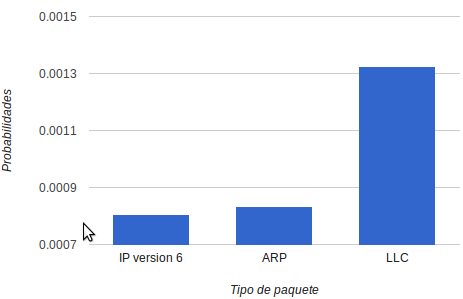
\includegraphics[width=0.5\textwidth]{exp1-graficos/grafico1exp1.png}
\end{center}

La entrop\'ia de la fuente S fue: 0.0337107429442.\newline

Dentro de los tipos ARP s\'olo capturamos 162 paquetes, como dijimos m\'as arriba. Era esperable, dado que el porcentaje presentado anteriormente era muy bajo con respecto al total. \newline
Vamos a analizar sobre estos, hacia que direcciones fueron enviados y que conclusiones obtenemos al respecto. Para eso podemos observar el siguiente histograma correspondiente a los IP destinos de los ARP, agrupados por la cantidad de veces que aparecieron durante la captura.

\begin{center}
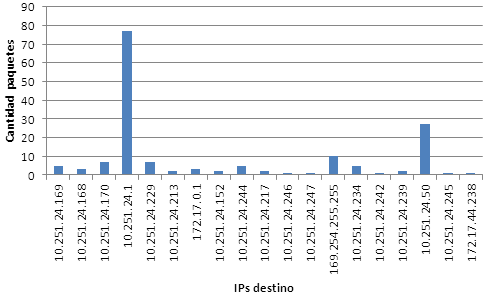
\includegraphics[width=0.75\textwidth]{exp1-graficos/grafico2exp1.png}
\end{center}

La entrop\'ia de la fuente S1 fue: 2.79796437031.


\subsubsection{An\'alisis de la captura}

1ra fuente:\newline

Como sabemos encontramos paquetes IPv6, ARP, LLC y DOD. DOD refiere a un paquete IPv4, asi que vamos a referirnos a \'el de ese modo.\newline

Podemos notar que las IPv4 y IPv6 consumen el 99\% de los paquetes, eso se debe a que hay un gran tr\'afico de paquetes de datos. Sin embargo el porcentaje de ARP es 0.08\%, muy bajo dado que se ha manejado un volumen de paquetes importantes (382.980 en total). Intuimos que esto se debe a que la topología de la red no sufre mucha variaciones, en consecuencia a que a cada dispositivo se le asigna una IP determinada a la hora de conectarse y no va a cambiar. Otro porcentaje un poco más alto que el de los ARP es el corresponde a los LLC (Logic Link Control) que maneja el control de errores, control del flujo, entre otras cosas.\newline

La entropía de la fuente $S$ es 0.0337.\newline

2da fuente:\newline

Dentro de los paquetes ARP podemos ver que se encuentran, en su mayoria, direcciones IP dentro de la red 10.251.24. Sin ser tan especificos notamos tres tipos de IP's, las iniciadas con 10, las iniciadas con 169 y las iniciadas con 172. Las iniciadas con 10 describen a una red simple clase A y determinan un bloque de 24bits. Las iniciadas con 172 describen a 16 redes clase B continuas. Y las inciadas en 169 describen a una red simple clase B no enrutable.\newline

Pudimos notar que nuestra notebook tenía un IP correspondiente a la red 10.251.24, por lo que concluimos que el resto de las ip correspondiente a esa red son celulares y pc's de la gente que estaba en el Starbucks en ese momento. Pudimos notar una IP reservada, 169.254.255.255. Y, dado la cantidad de paquetes que recibió (casi el 50\% del total, mirar histograma) y por la particularidad de su IP, pudimos notar que la dirección 10.251.24.1 refiere al IP del router de la red.\newline

La entropía de la fuente $S_1$ es 2.797.\newline




%Sniff de Stratbucks, el viernes.

%Paquetes vistos: 382980

%Probabilidad de IP version 6: 0.00080421954149
%Probabilidad de ARP: 0.000832941667972
%Probabilidad de LLC: 0.00132382892057
%Probabilidad de DOD Internet Protocol (IP): 0.99703900987
%Entropia de S: 0.0337107429442

%Paquetes ARP vistos: 162

%Probabilidad de 10.251.24.169: 0.0308641975309 - Paquetes: 5
%Probabilidad de 10.251.24.168: 0.0185185185185 - Paquetes: 3
%Probabilidad de 10.251.24.170: 0.0432098765432 - Paquetes: 7
%Probabilidad de 10.251.24.1: 0.475308641975 - Paquetes: 77
%Probabilidad de 10.251.24.229: 0.0432098765432 - Paquetes: 7
%Probabilidad de 10.251.24.213: 0.0123456790123 - Paquetes: 2
%Probabilidad de 172.17.0.1: 0.0185185185185 - Paquetes: 3
%Probabilidad de 10.251.24.152: 0.0123456790123 - Paquetes: 2
%Probabilidad de 10.251.24.244: 0.0308641975309 - Paquetes: 5
%Probabilidad de 10.251.24.217: 0.0123456790123 - Paquetes: 2
%Probabilidad de 10.251.24.246: 0.00617283950617 - Paquetes: 1
%Probabilidad de 10.251.24.247: 0.00617283950617 - Paquetes: 1
%Probabilidad de 169.254.255.255: 0.0617283950617 - Paquetes: 10
%Probabilidad de 10.251.24.234: 0.0308641975309 - Paquetes: 5
%Probabilidad de 10.251.24.242: 0.00617283950617 - Paquetes: 1
%Probabilidad de 10.251.24.239: 0.0123456790123 - Paquetes: 2
%Probabilidad de 10.251.24.50: 0.166666666667 - Paquetes: 27
%Probabilidad de 10.251.24.245: 0.00617283950617 - Paquetes: 1
%Probabilidad de 172.17.44.238: 0.00617283950617 - Paquetes: 1
%Entropia de S_1: 2.79796437031
